\chapter{CSS Intro \& Overview}
\label{css}
\paragraph{} In this chapter we begin to look at a second Web language, Cascading Style Sheets (CSS). This language is frequently considered to be a design or presentation language, and we'll start to look at how we can use CSS to style the elements of our HTML documents to make them look more visually appealing. HTML alone is really great, but pretty ugly. CSS gives us a way to improve how the elements of our pages are presented.

\section{HTML  \& CSS}
\paragraph{} As we've seen in the last unit, HTML gives us a language for describing structure. This is essential, without structure, our text loses its hypertext abilities, and the advantages gained from markup. However, we've also seen that, over time, HTML has had its abilities to define style, the presentation of the content, curtailed and in some cases removed. At the very least, using HTML's residual style capabilities to determine how a page should look is considered, at best, old fashioned and to be frowned upon.
\paragraph{} Instead, we now use a style language to determine how our content should appear. It is Cascading Style Sheets (CSS) that enable us to control presentation. This is not just about making things look pretty however, but is very important to usability and accessibility. Partly this is for the developers, instead of having content and presentation mixed they can be handled separately, perhaps by different members of the team. It also enables more efficient representation, for example, a style can be defined once and then applied wherever it is needed. 
\paragraph{} In addition, multiple different presentations of a single set of content can be defined and then used depending upon the context. This is how things like a print layout and a screen layout can be defined differently, or perhaps different screen layouts for different sizes of screen.
\paragraph{} In this unit we will concentrate on presentation from a technical perspective and specifically on how to style the individual elements of pages. We’ll then look at aspects of design over the next couple of units to try to apply this to produce cohesive designs. Briefly, styling individual elements (this unit), arranging groups of elements (next unit), and bringing everything together to create cohesive designs (next unit but one).


\section{HTML Content \& Presentation}
\paragraph{} Early versions of HTML mixed content and presentation. This was fine, it worked, but as the Web grew in capability and utility, the ways that the Web was used changed and this put pressures on design decisions made early on that governed the production of early websites. Initially every element needed font, colour, style, alignment, border, size, etc. to be explicitly described, often repeatedly so, throughout the HTML document. Anything that wasn't specified would revert to the default presentation. 
\paragraph{} Why does it default and where does the default style come from? To answer this it's worth noting that browsers have a built in style sheet that applies a default style to pages when no other style information is supplied. All style information, whether from HTML, or CSS, will override this internal browser stylesheet but in certain circumstances an end user will want to apply their own stylesheets to your site, regardless of your design. This is because end users might have their own accessibility requirements which must always take precedence over the web designers desires. The consequence is that you cannot rely on your carefully implemented design being what your user eventually sees. It is still worth caring that your default site is good and usable, but you should also ensure that the content is complete and well structured and not dependent upon the design for it to be usable.
\paragraph{} Over time, HTML has had its capabilities to describe style reduced. Moving style declarations, initially into their own separate blocks within the HTML document, and then later to external files made things both more simple, more efficient, and more flexible. The style declarations that were initially applied to typographical elements were eventually developed into a complete language for describing how HTML should be presented visually. These style declarations can now, with some caveats, be applied fairly uniformly across most HTML elements, not just applied to typographical elements. This allows not only a section of text to be styled, but also the block that it is grouped in, and every other element that makes up a given page.
\paragraph{} Overall, removing style declarations gives simpler HTML which can focus on content representation, structure, and semantics, and makes for more manageable designs. This is important once our sites begin to grow and become more complex.


\section{Content \& Presentation: A Separation of Concerns}
\paragraph{} Before getting into the technical aspects of CSS, let's consider a few important design related topics first, namely, the relationship between content and presentation. When we have HTML and CSS, and when applied properly, the visual and design aspects of a particular view, rendering, or usage of a document are separated from the core content and structure of that document.
\paragraph{} It's worth considering some other perspectives on the separation of content and presentation. Think of the human body. We have a skeleton which gives us structure but it is our flesh that gives us our appearance. Given a body without flesh, i.e. a skeleton, it is quite difficult for most people to distinguish this from any other skeleton, unless perhaps you are an anthropologist or physiologist. Similarly flesh without a skeleton would look and act very different. The two need to work together to give the individually distinguishable and capable humans around us, different complex systems working in concert. The same relationship holds between content and presentation, and between HTML (content) and CSS (presentation). Either, without the other, is less good than both working together.
\paragraph{} The nature of many modern, complex, computational systems means that a team of people work together on them. There are many tools for supporting co-operative work, but the separation of concerns, in this case the separation of content and presentation is of particular importance. By separating responsibilities it enables people to work in parallel, each working on their area separately to make progress. This doesn't mean working in isolation, just that the better separated the concerns, the more work can be done on each before progress on one is hindered by the other.
\paragraph{} This is not a rigid rule though, but more of a best practice. Different members of a team can work on each aspect and content can be presented in different ways. 
\paragraph{} This approach also has benefits after a site is deployed. It enables, for example, people with visual impairments to provide their own stylesheets to the browser to override the website developer’s decisions. It enables screen and print versions of pages to be styled differently. Content can be tailored to the medium of consumption.
\paragraph{} As I mentioned earlier, this is not a rigid rule, inline and embedded styles will work in most browsers, and you might not be able to tell the difference, and this is often useful for quick hacks when developing and trying to get things right. However this can lead to future problems. Separation of concerns leads to simplified change management, increased flexibility, and better usability.


\section{Design First or Content First?}
\paragraph{} This separation of concerns does raise a question though, should we design how our page will look first or create and structure the content first?
\paragraph{} Often you'll have a general idea for the overall look of a site before you start building it. At least you will usually have some idea of the feel that you are aiming for. Frequently this will be out of your control though, especially when building sites for others. Generally though you can’t really design something well until you have some idea of what the design is working with. You need some content or at least an idea of the structure of the content to get started with a design. Without content, the design might include things that won't appear in the site. At best, this is wasted effort, at worst, it can guide the design process in a direction that is wrong for the site you are building.
\paragraph{} We should recognise that content often drives the design process. Even without a design, we can take out content, structure and mark it up using HTML, and view this in a browser. We can have a navigable site without any design. It will certainly look quite poor though and will almost definitely not be anything like you would want to build, but it is a starting place. From this we can conclude that, if in doubt, we can start building the HTML, ensuring that it is well structured and captures all of the available content, before we start designing.
\paragraph{} Note that we can also start by mocking up the content. We'll see some techniques for doing this in the design for hackers unit. This is a great way to give you something that you can then start applying designs to. However, it is very likely that mocked up content will diverge widely from the final content which gives an opportunity for the design process to again head in the wrong direction. The need for mocked up content can occur in real world projects for many reasons though, often related to timing and imperfect alignment between business units. If the content writers are not yet ready to provide content, but the design and implementation teams are ready to start then it can be better to have them producing potential solutions that can later be verified using real content.
\paragraph{} We can relate this idea of a content first design process to other design ideas. For example, it is often said that ``Form follows function''. How something is structured stems primarily from the underlying engineering requirements and a desirable, often elegant, design is often the one that supports the needed functionality and nothing more where every extraneous element that is merely there for decoration has been pared away. Another way to think about content and design is 
to consider that we should not conform structure of content for design reasons if it then leads to a compromised system. If the design, for purely design reasons, then leads to a buggy, inefficient, unreliable, or unusable site, then something has gone wrong in the process. That said, we can, and indeed should, let structure inform the design process. Many elegant solutions stem from the design exposing underlying structure.
\paragraph{} If in doubt though, the default should be to start with content, write HTML, and think about your data before getting to design and CSS.



\section{An Overview of Cascading Style Sheets (CSS)}
\paragraph{} Having considered some important design considerations let’s now turn our attention more fully to the idea of CSS as a technology, before looking at the technical link between HTML and CSS. We'll then finish by looking in detail at CSS as a language.
\paragraph{} CSS is a simple, text-based, page appearance description language. In more formal terms we could also call CSS a declarative, domain-specific, programming language. These two descriptions give us lots of ways to consider what CSS is. We'll perhaps skip over the simple part for now. CSS documents can become quite complex if you write them that way, and you'll see lots of complex CSS in the real world, but there is no need for your CSS code to be complex. It can be simple and straightforward, but like most code, this property is mostly on the shoulders of the programmer. Text based indicates that, like HTML, it can be written using a standard text editor. No special tools are required. This contributes to the democratic nature of web technologies in general, most people can create the basic files that make up a web page without undue expense or effort. The "page appearance description language" phrase is useful though. It kind of sums up much of what CSS is about. It is a programming language for describing how a page should look. For our purposes the page is written using HTML so CSS is describing how an HTML page should appear when rendered.
\paragraph{} In the more formal description we had the term "declarative". This term implies that control flow is implicit. We are saying what we want and the computer then tries to achieve that. We don't say exactly how the end result should be achieved we just declare what we want. This leads us to thinking of CSS as a constraint language. The browser, when rendering, can do what it likes to our HTML page. It generally doesn't, but it can. By using CSS we are declaring what we want the browser to try to achieve by imposing constraints on the elements that make up the page. For example, a declaration that a section of text should be red is also imposing a constraint on the range of valid colours for that section of text. This is also where some of the potential complexity of CSS arises. Some constraints can be incompatible, if we declare that we want to make a section of text bigger, then the container in which the text is held must grow to still be able to contain it. If we also constrain the size of the container then there will be conflict and the effect as a result can be different, for example, either one of the declarations is overridden, the container can grow to enclose the text, or else the text can spill out of the container or be clipped at the edge of the container. This is where some of the perceived complexity of CSS can stem from.
\paragraph{} However HTML and CSS are resilient. If a browser can’t do what you declare in the CSS then the site will generally continue to function. It is rare for the content to fail to be displayed at all. But it might be unlike the designer intended.
\paragraph{} CSS permits almost every HTML tag to be arbitrarily scaled, positioned, and decorated. This overcomes some limitations of styling associated with traditional HTML because HTML limits the application of styles to particular, usually typographical, elements. However, we shouldn't think of CSS as a pixel-perfect user interface design tool like we might use for building desktop or mobile apps. It is not. It is better considered as a tool that enables flexible and robust user interfaces to be implemented that will reflow to work well with screens of different sizes across many platforms.



\section{The Slow Detachment of Style and Presentation from Content}
\paragraph{} Let's now quickly survey how the detachment of presentation from content has occurred in HTML. We've moved from the pre-CSS HTML presentational attributes, for example,

\begin{lstlisting}
<h1><font color=“red”>The Quick Brown Fox</font></h1>
\end{lstlisting}

\paragraph{} to the use of style parameters such as,

\begin{lstlisting}
<h1 style="color: red;”>The Quick Brown Fox</h1>
\end{lstlisting}

\paragraph{} Because style parameters only apply to the elements to which they are attached, meaning that declarations with similar parameters might need to be repeated in many places in the same file, a more efficient solution was required. We moved to style blocks, collecting style declarations in their own area of the HTML document, separated from the HTML elements to which they are applied. For example,

\begin{lstlisting}
<!DOCTYPE html>
<html>
	<head>
		<style type=“text/css”>
			h1 {color: red;}
		</style>
	</head>
	<body>
		<h1>The Quick Brown Fox</h1>
	</body>
</html>
\end{lstlisting}

\paragraph{} The limitation of style blocks is that a given block only applies to that one page that it appears to. However we likely want our entire site to have a similar and consistent style across all pages. So why not collect styles into an external, separate file, and then include it wherever it needs to be used. This leads to external style sheets. Here is an example of the line that would be included in an HTML file to tell it where to find a CSS file for use:

\begin{lstlisting}  
<link href="path/to/file.css" rel="stylesheet" type="text/css">
\end{lstlisting}

\paragraph{} Best practice is to use an external stylesheet.


\section{Using CSS \& HTML Together}
\paragraph{} In the modern web, CSS can be used with HTML in 3 primary ways which are very similar to what we've just seen. Considering the previous topic, the only approach that is no longer valid is the earliest, using presentational attributes. All three others are valid in the modern web but have various advantages and disadvantages. We can

\begin{enumerate}
	\item Attach CSS to a specific HTML element using the style parameter.
	\item Inline CSS globally by collecting it together using a <style> block
    \item Retrieve CSS from an external URL using directives like this:
\end{enumerate}

\begin{lstlisting}
<link rel="stylesheet" type="text/css" href=“theme.css”>
\end{lstlisting}

\paragraph{} We'll look at each of these in turn over the next three topics and consider the advantages and disadvantages of each.


\section{Using the Style Parameter}
\paragraph{} The style parameter is used "inline"  as an attribute of the HTML Element to which it is applied

\begin{lstlisting}
<p style=“color:red”>
\end{lstlisting}

\paragraph{} An advantage of this is that you can put your style declarations right where you’re using them. You don't have to scroll to a different part of the file or look in a separate file, it is right there. However, this can lead to lots of repetition. You have to specify everything exactly where you want it. For example, every paragraph that you want to colour red must have an inline declaration which can seriously bloat your site. This is also an extreme mixture of content and presentation. There is no real separation between the two when taking this approach.


\section{Using a $<$style$>$ block}
\paragraph{} A style block enables us to collect all of the style declarations together, for example, those that we might have attached otherwise to individual HTML elements. This means that you can make a single declaration, e.g. color: red; and then list all of the places that it should be applied to. For example,

\begin{lstlisting}
<!DOCTYPE html>
<html>
	<head>
		<style type=“text/css”>
			h1 {color: red;}
		</style>
	</head>
	<body>
		<h1>The Quick Brown Fox</h1>
	</body>
</html>
\end{lstlisting}


\paragraph{} Here we have a style block in the head section of the HTML document. There is a single declaration, color:red; and this is applied to a single HTML element, the $<$h1$>$ tag.

\paragraph{} This begins to separate presentation from content. The content is all in the <body> section of the document and the style is now separated into the style block in the <head> section.

\paragraph{} However, this only styles individual pages and not sites. To style all pages in a site using this approach requires the style block to be repeated in every page. If we then make a change to the design, we must edit all style blocks in all pages to ensure consistency across the site.

\section{External Stylesheets}
\paragraph{} External stylesheets give us the ultimate, so far, in separation of content from presentation. Content is now stored in the relevant HTML files and styles are stored in CSS files. Multiple HTML files reference the CSS file and hence the style for the site only needs to be placed in a single place, and only needs to be updated in a single place. In other words, we can reuse the same .css file in multiple .html files. This enables us to style an entire site (multiple HTML files) with all the CSS declarations for the visual presentation of the site in one place. This is reasonably easy to manage and update the design without touching the content. We can also add new content and take advantage of a ready made style.  Let's look at how this works in practice. Here are the contents of two files, index.html and style.css which work together to style the content of a simple page:

	index.html

\begin{lstlisting}
<!DOCTYPE html>
<html>
	<head>
		<link href=“style.css" rel="stylesheet" type=“text/css" media=“screen”>
	</head>
	<body>
		<h1>The Quick Brown Fox</h1>
	</body>
</html>
\end{lstlisting}

\paragraph{} and the CSS (style.css):

\begin{lstlisting}
body {background-color:black}
h1 {color:red}
p {color:blue}
\end{lstlisting}

\paragraph{} Notice that the $<$link$>$ element in the HTML document references the name of the stylesheet. This is how we tell an HTML page which stylesheet to use. Within the stylesheet, notice that it references HTML elements that exist in the HTML file. So these two files aren't completely separate. The CSS must declare styles for elements that exist in the HTML document else there is nothing to style. Similarly, to take advantage of a style, the HTML document must include elements that are declared in the CSS.

\paragraph{} It is this that enables us to take advantage of ready made CSS designs. There are lots of ready made style collections available, under a variety of licenses that can be included into your HTML. This can mean that you can avoid writing any CSS if you are happy to adopt an existing design and to perhaps have a site whose look and feel is shared with other sites. We'll consider this in more detail in the design for hackers unit.

\paragraph{} We should also note that another advantage of external stylesheets is that a page can specify multiple different stylesheets which can be applied in different contexts. A common one that you might have experienced is when printing a page you might notice that the printed layout can differ from the on-screen layout. Similarly, many sites now have dark and light modes which switch depending upon ambient light conditions, or user preference. These are all controlled and defined through the provision of stylesheets for each context. The HTML media attribute lets you specify different style sheets for different contexts, e.g. print, projection, aural, braille, tty, tv, etc.



\section{Basic CSS Syntax}
\paragraph{} So far we've looked at how CSS is related to HTML, how CSS expressions can be made available to an HTML document through inlining, blocks, or external files. However we've not really looked at the language itself yet. Let's remedy that.
\paragraph{} CSS is used to write stylesheets and stylesheets are merely a list of rules that declare how we want particular HTML elements to be styled. The rules are constructed from selectors and declarations.
\paragraph{} Selectors are used to find relevant HTML elements to apply the declaration to. The declaration is a list of simple pairs of property and value. Each element of the list is separated by semi-colons and properties are delineated from values using colons. This is illustrated in the following figure:


\begin{figure}[H]
\centering
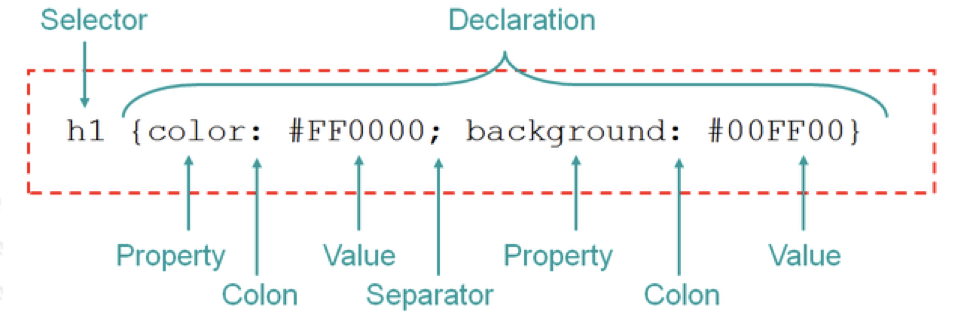
\includegraphics[width=0.8\textwidth]{figures/css-syntax}
\label{fig:css-syntax}
\caption{}
\end{figure}


\paragraph{} CSS rules use a simple syntax and are fairly easy to understand. Essentially one or more selectors identify which html elements to target then a declaration specified how to style those elements.


\section{Selectors}
\paragraph{} We use selectors in CSS to tell the browser which parts of the markup to apply a style to. For example we can tell the browser to apply a style to all instances of a given HTML element within a document, e.g. $<$h1$>$ or $<$img$>$.
\paragraph{} Sometimes though we will want to treat different instances of the same element in different ways, for example, style the first paragraph in one way and other paragraphs in another way. To support this CSS has a few ways to target different groups of elements or even individual elements. Recall that we can give an HTML element a unique ID attribute to enable us to differentiate that single element from all of the others. In CSS we target elements with a specific ID attribute, e.g. $<$p id=``para-123''$>$, using a selector that matches the ID, e.g. \#para-123.
\paragraph{} Sometimes though we don't want to target just an individual, and we don't want to target just a given element, what we want to do is to target an arbitrary group of elements. We can do this using the class attribute. If the element has the matching class attribute defined, then it will be matched by the selector, e.g. We can use the .photos selector to match elements in our HTML document that  have the same class, e.g. $<$p class=``photos''$>$. 
\paragraph{} Note that there are also so-called pseudo-classes which refer to special states of selected elements, e.g. hover, visited, active, \&c. Pseudo-classes enable elements to be styled in relation to things outside the DOM, e.g. the history of navigation or whether a link has previously been interacted with or followed. We can combine and join selectors  in many ways to specify elements by location, element type, id, class (or any combination thereof).



\section{Declarations}
\paragraph{} As we saw in the CSS syntax topic, declarations work with selectors. One to tell the browser which elements to target and the other to tell the browser the set of properties to apply to the elements so selected.
\paragraph{} Individual declarations are relatively simple. They are designed to give a specific value to a property. This is what is known more widely as a key:value pair. A declaration comprises a property, a colon (:), and a value, e.g. {\emph{color: red}}.
\paragraph{} Properties are defined in the CSS standard and each property has a given set, or range, of legal values. These can include keywords like ``center'' or values such as numeric values, percentages or others. For example, colour can be specified with keywords, e.g. ``red;;, or Hex values  like \#FF0000 or RGB values like rgb(255, 0, 0).
\paragraph{} It is worth getting used to consulting documentation when it comes to CSS properties and values. Some CSS properties can affect any type of element whereas other properties can apply only to particular groups of elements.
\paragraph{} Because we are likely to want to set multiple properties efficiently, a declaration is really a semi-colon separated list of multiple individual declarations (key-value pairs). For example, here are two declarations separated by a semi-colon:

\begin{lstlisting}
color: red; text-align: center;
\end{lstlisting}

\paragraph{} When using declarations in a CSS file we enclose them into a declaration block, a list of declarations encapsulated between braces, like so:

\begin{lstlisting}
	h1 {color: red; text-align: center;}
\end{lstlisting}

\paragraph{} The takeaway from this should be that CSS declarations are quite straightforward and don't have to be complex or unwieldy. The trick is for you, as the developer, to stay in control.



\section{CSS Design Constraints}
\paragraph{} CSS applies styling and layout to HTML elements, it doesn't create them. We can use CSS to declare that we want to paint a border around an HTML element but we cannot create the basic element itself in pure CSS. All we are doing with CSS is declaring how the page should be displayed but the actual display of the page is the responsibility of the browser and its layout engine. The layout engine will attempt to consistently apply all of the constraints imposed by the CSS onto the elements defined by the HTML. If there are mutual incompatible constraints then these will be resolved by the rules written into the layout engine and this is highly dependent upon the order in which the constraints are imposed with the CSS file.
\paragraph{} The idea is that CSS can be used to describe various layouts of content. When the browser layout engine renders this content, it takes account of the platform it is running on and adjusts things as a result. This is how web pages can adjust automatically to any screen/viewport/canvas on any platform. CSS, HTML, and browsers are designed to do this, which is one of the reasons why they are less accomplished when trying built pixel-perfect interfaces. For example, web pages give us text that scales independently of the viewport. Scaling a font, i.e. making text bigger, should lead to a reflow of the page content, shifting other things further down the page to make space, it shouldn't lead to horizontal scrolling. Many browsers also use progressive rendering. In any given page, the layout depends on previous content, i.e. content further up the page, but not future content. However, loading new content might force a reflow of previously rendered content. For example, consider if there is an image element tag part way down a page. If the element doesn't specify the dimensions of the image then space can't be left for the image until it is fully loaded, but this might hold up displaying the rest of the page. Many users would prefer to be able to see the content of a page as it loads, especially the words, rather than waiting for everything to be complete. So the browser will display what it has, then re-render the page if necessary as elements finish loading.
\paragraph{} A reminder though that the user can override anything regardless of what the designer thinks or intends. Once your HTML and CSS reach the user’s browser, the user is in control. There are valid reasons for this as we explored earlier, mainly to do with accessibility and enabling the user to choose how to consume their data.



\section{Inheritance}
\paragraph{} Inheritance, the idea that we can build on pre-existing CSS declarations is a key CSS feature. The idea is that we should be able to take advantage of the existence of hierarchical structure in HTML documents to make things more efficient.
\paragraph{} Recall that HTML is parsed into the DOM, a model of the objects that make up a page. The DOM is a tree and is therefore hierarchical. It starts with the root $<$html$>$ tags and all page content is encapsulated within that. When styles are applied to elements higher up the DOM hierarchy they can be inherited by elements further down the hierarchy. In this way nested descendants generally inherit text-related properties from parent elements that enclose them. This is efficient because we then don’t have to declare the same properties repeatedly at each level of the DOM hierarchy. For example, given:

\begin{lstlisting}
	<h1>
	   This is to $<$em>illustrate</em$>$ inheritance
	</h1>
\end{lstlisting}

\paragraph{} and the following style declaration:

\begin{lstlisting}
h1 { color: purple; }
\end{lstlisting}

\paragraph{} But no declaration for the colour of the $<$em$>$ element, the $<$em$>$ element would inherit the h1 property without us needing to explicitly declare that the word "illustrate" between the $<$em$>$ tags should also be coloured purple.

\paragraph{} Admittedly, this is one of the areas of CSS that causes confusion in practice. It can be difficult to determine where exactly an inherited style comes from even when examining the DOM through the browser developer tools.



\section{Colours}
\paragraph{} Colour is an easy place to start when thinking about styles. It has visual impact greater than most other aspects of style. We can control the colour of an element by using the ``color'' property. We've seen the color property used in several of the examples so far, e.g.

\begin{lstlisting}
h1 { color: purple; }
\end{lstlisting}

\paragraph{} to set the color property of the h1 element to purple. There are however 140 named colours in CSS which we can use directly just by supplying the name as the value to the color property. These include the following: \emph{lightcoral, rosybrown, indianred, red, firebrick, brown, darkred, maroon, mistyrose, salmon, tomato, darksalmon, coral, orangered, lightsalmon, sienna, seashell, chocolate, saddlebrown, sandybrown, peachpuff, peru, linen, bisque, darkorange, burlywood, antiquewhite, tan, navajowhite, blanchedalmond, papayawhip, moccasin, orange, wheat, oldlace, floralwhite, darkgoldenrod, goldenrod, cornsilk, gold, lemonchiffon, khaki, palegoldenrod, darkkhaki, ivory, lightyellow, beige, lightgoldenrodyellow, yellow, olive, olivedrab, yellowgreen, darkolivegreen, greenyellow, chartreuse, lawngreen, darkseagreen, honeydew, palegreen, lightgreen, lime, limegreen, forestgreen, green, darkgreen, seagreen, mediumseagreen, springgreen, mintcream, mediumspringgreen, mediumaquamarine, aquamarine, turquoise, lightseagreen, mediumturquoise, azure, lightcyan, paleturquoise, aqua, cyan, darkcyan, teal, darkslategray, darkturquoise, cadetblue, powderblue, lightblue, deepskyblue, skyblue, lightskyblue, steelblue, aliceblue, dodgerblue, lightslategray, slategray, lightsteelblue, cornflowerblue, royalblue, ghostwhite, lavender, blue, mediumblue, darkblue, midnightblue, navy, slateblue, darkslateblue, mediumslateblue, mediumpurple, blueviolet, indigo, darkorchid, darkviolet, mediumorchid, thistle, plum, violet, fuchsia, magenta, darkmagenta, purple, orchid, mediumvioletred, deeppink, hotpink, lavenderblush, palevioletred, crimson, pink, lightpink, white, snow, whitesmoke, gainsboro, lightgray, silver, darkgray, gray, dimgray, black.}

\paragraph{} Colours can be referred to by name, at least for the 140 named colours, but also by hex code, RGB or HSL code. When using hex, RGB, or HSL codes then there are many more than 140 colours available and you have full access to a space of approximately 16M+ colours.


\section{Background}
 to set the color property of the h1 element to purple. There are however 140 named colours in CSS whiAfter colour, interacting with the background of the web page is probably the most prevalent way to alter the stylistic character of a page. An easy way is through the background-color property. We can supply it with any of the named colours or colour codes covered in the last topic. Alternatively, we supply an image to be set as the value of the background-image property. This is a picture that is used behind the text and other elements that make up the page content. Background images can be manipulated in various ways, for example being made to repeat, e.g.

\begin{lstlisting}
background-repeat \{repeat, repeat-x, repeat-y, no-repeat\}
\end{lstlisting}


 to set the color property of the h1 element to purple. There are however 140 named colours in CSS whior for the image to be located in specific places using the background-position property:

\begin{lstlisting}
background-position - specify two values for horizontal and vertical from \{top, bottom, left, right, center\}
\end{lstlisting}
	

\section{Font Properties}
\paragraph{} After the page background, the typographical elements of the page content are the next most prevalent elements that are styled. We can style the following:

\begin{itemize}
	\item font-family - which font to use
	\item font-size - how big it should be
	\item font-style - \{normal, italic, oblique\}
	\item font-weight - \{normal, bold, bolder, lighter, +numeric values\}
\end{itemize}



\section{Text Properties}
\paragraph{} When dealing with typographical aspects of page content, it is not only the fonts that are important to consider, but also the properties of the text itself, regardless of the font and how the letters themselves are displayed. Think about when word processing a document, you will frequently use the text alignment to left or right align your text, as well as decorators, perhaps to underline certain sections of text. CSS enables us to style our page content in similar ways:

\begin{itemize}
	\item text-align - justify blocks of text, e.g. \{left, right, center, justify\}
	\item text-decoration - \{none, underline, overline, line-through, blink\}
	\item text-transform - \{non, capitalize, uppercase, lowercase\}
\end{itemize}



\section{Links}
\paragraph{} I've already belaboured the importance of links in the process of turning text into hypertext. It would be a huge omission if we couldn't also control how we want links to be displayed in our pages. CSS gives us this control and we can affect the color and text properties of links using the following selectors:

\begin{itemize}
	\item link - the normal state
	\item visited - if the link has previously been followed
	\item hover - while pointer is over link
	\item active - whilst being clicked
\end{itemize}

\paragraph{} These enable us to define how links should look in their various states, e.g. 

\begin{lstlisting}
a:link {color:red}
\end{lstlisting}

\paragraph{} declares that we want to select the hyperlinks that are in their normal state, i.e. not previously visited or currently actively engaged with by the user. Having selected these links, we want to set their color property, e.g. the colour of their text, to red. Many implemented sites will choose a palette of link colours that work well with the design of the site.



\section{The Box Model}
\paragraph{} You might be wondering at this point how the browser places all of these differently shaped elements onto a web page when it is rendering it. The secret is the CSS box model. This places every element of content into a set of boxes that affect spacing and placement in relation to all of the other elements of the page and their CSS declarations in turn. At this point you should be starting to appreciate just how complex the interactions between HTML, DOM, CSS and layout/rendering engine can become.
\paragraph{} The box model defines the following:

\begin{itemize}
	\item Padding - distance between edge of element and its content 
	\item Border - frontier between padding and margin
	\item Margin - distance between edge of element and adjacent element
\end{itemize}

\paragraph{} which can be used to control the space around an element in a number of contexts. These are illustrated in the following figure:

\begin{figure}[H]
\centering
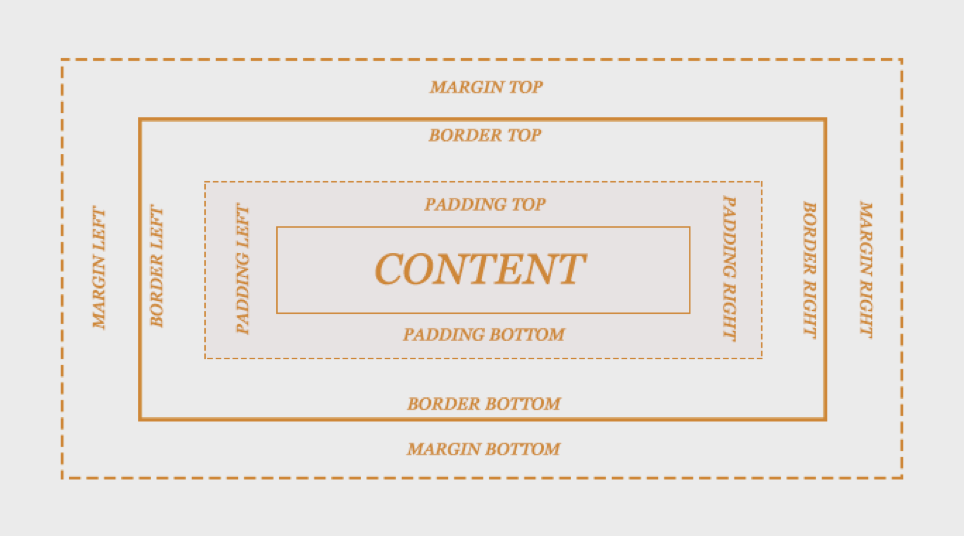
\includegraphics[width=0.8\textwidth]{figures/box-model}
\label{fig:box-model}
\caption{}
\end{figure}


\paragraph{} Notice that padding, border, and margin are divided into four edges, because they are boxes around the content element, the edges are top, bottom, left, and right. Applied to the border element gives us:
	border-left, border-right, border-top and border-bottom 

\paragraph{} The same naming pattern works for the margin and padding boxes. Boxes also have borders which can be visually styled. Often setting them to none is preferred, but borders can be applied to all edges or to individual edges, specifying border characteristics, e.g. {solid, dotted, dashed, double} as well as width and colour.



\section{Browser Rendering \& CSS}
\paragraph{} We've mentioned before some aspects of the job that the browser does in rendering the static HTML and CSS files into a visual representation on screen. Much of this occurs automatically according to the rules of the specific rendering engine used by the user's browser. However, some elements of the rendering process can also be manipulated through CSS. How the browser lays out HTML elements follows from the constraints declared in the CSS associated with the page. 
\paragraph{} However we can use the display property to affect the rendering of specific elements. For example, 

\begin{itemize}
	\item inline - Elements flow horizontally left to right as space allows. Line breaks happen when the edge of the container is reached, and the flow continues on the next line.
	\item block - Elements flow top down, one after another. The width of the block is what is available in the container, the height is defined by the content.
	\item table - Child elements are aligned both vertically and horizontally.
	\item flex - Child elements are placed on a single axis either vertically or horizontally, which specified alignment, adjustments and spacing.
\end{itemize}

\paragraph{} We shall examine the flex and table declarations in the next unit as they are very useful if we want to build particular layouts for our pages.



\section{Perceptions of CSS \& Getting the most from it}
\paragraph{} CSS is often perceived as being hard or difficult, but this is often due to thinking of CSS as something that it’s not. It is not, for example, a pixel perfect layout tool like we might see in the graphic design industry for laying out printed pages. It is wrong to think this way. If you instead think of it as a flexible way to produce pages that work in lots of contexts, arranging page content in near optimal ways to make it easy to consume from the widest range of devices and screens, then it starts to make more sense. We can't easily specify an exact layout for every possible screen, but we can declare our desires and then allow the browser to make the best job of arranging things on screen according to those declarations. The complexity in CSS stems from trying to exercise too much control over how the browser renders the page, requiring increasingly complex rules to govern all of the different exceptional states that might occur. As these start to add up we start to realise where the reputation for difficulty comes from. CSS rules can combine and be inherited in a page, and the more rules, the more likelihood for unintended interactions between rules.
\paragraph{} So perhaps a change in mindset is required when designing for the Web. We should want to develop sites that are of the web, not merely put on the web. Properties interact and can lead to unexpected results - set one and it combines with others (and defaults) so we perhaps should never be more explicit than necessary to get the effect we want. If we refrain from going too far down the page layout control route and trust our browser rendering engine to do its job, then HTML pages are responsive by default. So my advice is to work with this rather than against it and refrain from trying to force the rendering engine into different or overridden behaviour. Let your content determine either width or height (or both) instead of forcing dimensions and layouts. 
\paragraph{} Ultimately, as soon as you try to impose your will on how your content must be viewed in the users browser then you are setting up more work for yourself at the very least, and at worst causing problems for yourself where there need not be any.

\section{summary}
\paragraph{} You should now be able to explain why structure and presentation are treated separately, understand how HTML and CSS are related, and have a basic grasp of the syntax and semantics of CSS. As with HTML (and later Javascript) we have only scratched the surface of what each technology can do. This is a foundation. Exploring what it can do for you is your responsibility.

